\section{Wzroce projektowe (2) - strukturalne}

Strukturalne wzorce projektowe wyjaśniają jak łączyć obiekty i klasy w większe struktury zachowując jednocześnie prostotę i elastyczność.

\subsection{Adapter (ang. adapter)}\label{sec/lab3/adapter}

Wzorzec który pozwala na działanie dwóch komponentów o niezgodnych interfejsach nazywany jest Adapterem. Jeśli klasa potrzebuje do działania obiektu klasy o określonym interfejsie, natomiast klasa która mogłaby zostać wykorzystana posiada inny, niezgodny interfejs, można utworzyć klasę adaptera, która dostosuje niezgodne interfejsy. Stosuje się go do dopasowywania kodu, który już istnieje. Jest często wykorzystywany w~celu wykorzystania zewnętrznego zestawu firm trzecich np. pobranego z menadżera pakietów NuGet, którego interfejs jest niezgodny z tym używanym w naszej aplikacji.

\begin{figure}[hbt!]
	\centering
	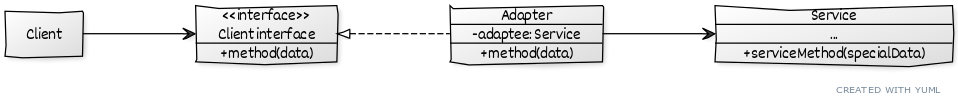
\includegraphics[width=0.9\linewidth]{images/AdapterUml}
	\caption{Diagram UML wzorca Adapter.}
	\label{lab3/fig/AdapterUml}
\end{figure}
%[Client interface]^-.-[Adapter]
%[Adapter]->[Service]
%[Client]->[Client interface]
%
%[Client]
%[<<interface>>Client interface|+method(data)]
%[Adapter|-adaptee: Service|+method(data)]
%[Service|...|+serviceMethod(specialData)]

Wyobraźmy sobie sytuację, w której mamy działający komponent i do logowania informacji o swoim działaniu wykorzystuje napisany przez nas zestaw np. bibliotekę. Klasa logera implementuje określony interfejs np. \texttt{ILogger}. Wykorzystując ten interfejs, klasa kliencka używa obiektu klasy logera do logowania. Jeśli za jakiś czas okaże się konieczne wykorzystanie bardziej rozbudowanego narzędzia do logowania np. pakietu NLog, możemy albo zmieniać odwołania w kodzie klienckim, albo wykorzystać wzorzec Adapter. W drugim przypadku adapterem będzie klasa implementująca nasz interfejs \texttt{ILogger} i posiadająca obiekt typu \texttt{NLog.Logger} przekazany/wstrzyknięty np. jako argument konstruktora. Wszystkie metody interfejsu \texttt{ILogger} są przekazywane do odpowiednich metod pakietu \texttt{NLog}. Po napisaniu adaptera wystarczy wstrzyknąć nowo utworzony obiekt do kodu klienckiego bez dodatkowych modyfikacji. Nie będzie również problemem napisanie dodatkowego adaptera dla innego pakietu np. Log4N. Ze względu na fakt, że oba adaptery implementują ten sam interfejs można napisać wiele różnych adapterów dla adaptowanych obiektów, które będą wykorzystywane przez kod kliencki.

%https://stackoverflow.com/questions/9892137/windsor-pulling-transient-objects-from-the-container/9915056#9915056
% Steven answer
%Należy mieć na względzie, że dobrze jest logować informacje w możliwie jak najmniejszej liczbie miejsc. Często warto jest stworzyć blok \texttt{try{}catch{}} na samym szczycie aplikacji i to w tym miejscu przechwytywać wszystkie wyjątki.

%https://docs.microsoft.com/en-us/aspnet/core/fundamentals/logging/?view=aspnetcore-5.0#console
%https://codewithmukesh.com/blog/logging-with-nlog-in-aspnet-core/
%https://stackoverflow.com/questions/5646820/logger-wrapper-best-practice
%https://stackoverflow.com/questions/41243485/simple-injector-register-iloggert-by-using-iloggerfactory-createloggert/41244169#41244169
%https://blog.stephencleary.com/2018/06/microsoft-extensions-logging-part-2-types.html

% Why use generic version of ILogger over non-generic one
%Quoting Steven's comments on this question: "Injection of a ILogger<T> is just noise to the consumer that can lead to accidental errors when a wrong T is specified and it complicates testing."... "Injecting ILoggerFactory and ILogger<T> is a terrible idea, and as I see it, the only reason Microsoft is doing this (and promoting it publicly) is because their built-in container lacks the possibility to map a non-generic interface to a generic implementation." – Hooman Bahreini Nov 26 '20 at 22:22

Innym przykładem zastosowania wzorca Adapter może być sytuacja w której posiadamy aplikację, która pobiera dane z plików tekstowych w formacie \texttt{XML} i następnie je przetwarza oraz wizualizuje te dane w formie wykresów. Z czasem może pojawić się potrzeba, aby dane pobierać z zewnętrznego serwera w innym formacie np. \texttt{JSON}, korzystając z gotowego zestawu (np. pakietu NuGet). Jeśli korzystamy z rozwiązań innych firm nie ma możliwość zmiany interfejsu zestawu pobierającego dane z serwera. Implementując wykorzystywany wcześniej interfejs możemy przekierowywać żądania od klienta do zewnętrznego zestawu ,,w locie'', zmieniając format danych z \texttt{XML} na \texttt{JSON}.

Opisana powyżej wersja adaptera jest wersją obiektową tego wzorca. Można się również spotkać z podejściem klasowym. W drugim podejściu obiekt adaptera zamiast posiadać adaptowany obiekt, może po nim dziedziczyć. Wersja obiektowa jest jednak częściej stosowana zgodnie z zasadą, aby przekładać kompozycję nad dziedziczenie.

% Plusem adaptera klasowego jest możliwość przesłonięcia składowych wirtualnych, abstrakcyjnych. 
% W przypadku C++ stosując adapter klasowy należy publicznie dziedziczyć po klasie Target oraz prywatnie po klasie Adaptee.
% Podejście obiektowe jednak pozwala na działanie jednej klasy Adapter z wieloma Adaptee

\subsubsection{Zadanie 1}
Celem tego zadania, będzie napisanie adaptera dla pakietu służącego do logowania informacji diagnostycznych w naszej aplikacji. Wykorzystany zostanie popularny pakiet NLog, który dostarcza bogaty zbiór różnych możliwości logowania m.in. komunikaty mogą być wyświetlane na ekranie konsoli, wysyłane mailem, zapisywane do pliku, bazy danych, czy chmury. Zastosowanie wzorca Adapter pozwoli nam na wykorzystanie tego pakietu, bez konieczności uzależnienia się od niego. Jeśli w przyszłości konieczne okaże się użycie np. Log4N zamiana będzie bardzo prosta.  

W pierwszej kolejności utwórz projekt aplikacji konsolowej .NET 5.0. Za pomocą menedżera pakietów dodaj pakiet NLog. Konfiguracja pakietu odbywa się z użyciem pliku NLog.config. Utwórz plik o takiej nazwie i~rozszerzaniu w~folderze projektu. Skopiuj do niego poniższe reguły logowania:
\begin{lstlisting}[caption={Konfiguracja pakietu NLog}, label={lab3/lst/nlogConfig}]
<?xml version="1.0" encoding="utf-8" ?>
<nlog xmlns="http://www.nlog-project.org/schemas/NLog.xsd"
xmlns:xsi="http://www.w3.org/2001/XMLSchema-instance">

	<targets>
		<target 
			name="_File" 
			xsi:type="File" 
			fileName="${basedir}/Logs/${shortdate}.log" 
			layout="${longdate}|${uppercase:${level}}: ${message}"/>
		<target 
			name="_Console" 
			xsi:type="Console" 
			layout="${longdate}|${uppercase:${level}}: ${message}"/>
	</targets>
	
	<rules>
		<logger name="*" minlevel="Info" writeTo="_Console" />
		<logger name="*" minlevel="Debug" writeTo="_File" />
	</rules>
</nlog>
\end{lstlisting}
Plik\ref{lab3/lst/nlogConfig} zawiera targety oraz reguły. Te pierwsze wskazują, w jaki sposób chcemy zapisać informacje\footnote{Targety pakietu NLog moją bardzo bogate możliwości parametryzacji. Szczegóły można znaleźć na wiki repozytorium pakietu: \url{https://github.com/nlog/NLog/wiki}}, w~przypadku naszej konfiguracji, będzie to wypisanie wiadomości na ekranie konsoli oraz zapisanie w pliku tekstowym. Reguły natomiast definiują jaki poziom ,,ważności'' informacji ma zostać zapisany w jakim targecie. Aby plik NLog.config mógł być wykorzystany konieczne jest jego przekopiowanie do folderu z plikiem wykonywalnym. Klikając PPM na nazwę pliku należy wybrać Properties i dalej w opcji Copy to Output Directory wskazać opcję Copy always. Dzięki temu w momencie kompilacji plik konfiguracyjny znajdujący się katalogu głównym projektu zostanie skopiowany do folderu z plikiem wykonywalnym.

Sprawdzić działanie pakietu NLog można pobierając instancję logera metodą \texttt{GetCurrentClassLogger()} w pokazany na listingu~\ref{lab3/lst/nlogPackageTest} sposób. Po uruchomieniu programu w folderze bin/Debug/Logs powinien pojawić się plik tekstowy *.log. Dodatkowo komunikaty powinny zostać wyświetlone na ekranie konsoli.
\begin{lstlisting}[caption={Wywołanie metod logujących pakietu NLog}, label={lab3/lst/nlogPackageTest}]
using NLog;

namespace AdapterDesignPattern
{
	class Program
	{
		private static readonly Logger Logger = LogManager.GetCurrentClassLogger();
		
		static void Main()
		{
			Logger.Info("Hello world");
			Logger.Error("Goodbye cruel world!");
			Console.ReadLine();
		}
	}
}
\end{lstlisting}


Załóżmy, że nasza aplikacja wymaga wykorzystania narzędzia logującego. W tym celu będziemy wykorzystywać własny, wcześniej zdefiniowany interfejs \texttt{ILogger}. Użycie własnej abstrakcji uniezależnia nas od konkretnego pakietu/zestawu. Będzie on deklarował następującego metody zwracające typ \texttt{void} i przyjmował argument typu \texttt{string}:
\begin{itemize}
	\item LogTrace
	\item LogDebug
	\item LogInformation
	\item LogWarning
	\item LogError
	\item LogCritical
\end{itemize}
Stwórz plik z powyższym interfejsem w osobnym pliku w~projekcie. 

Dodaj do projektu prostą klasę, która w konstruktorze będzie oczekiwała obiektu implementującego utworzony przed chwila interfejs \texttt{ILogger}. Klasa ta będzie klientem obiektu logera. 
\begin{lstlisting}[caption={Przykład klasy wykorzystującej obiekt klasy implementującej \texttt{ILogger}}, label={lab3/lst/customControllerWithLogger}]
public class CustomController
{
	private readonly ILogger logger;
	public CustomController(ILogger logger) => this.logger = logger;
	public void Get() => logger.LogInformation("API request");
}
\end{lstlisting}

Nie możemy przekazać logera NLog do obiektu typu \texttt{CustomController} ze względu na niezgodne interfejsy. Aby je dopasować wykorzystamy wzorzec projektowy Adapter. Dodaj do projektu klasę \texttt{NLogAdapter}. Klasa musi posiadać referencję do obiektu, który adaptuje. Zostało to pokazane na diagramie UML\ref{lab3/fig/AdapterUml}. W~tym przypadku będzie to klasa \texttt{Logger} pakietu NLog. W~klasie adaptera dodaj konstruktor z parametrem typu \texttt{NLog.Logger}. Dodatkowo klasa powinna implementować interfejs \texttt{ILogger}. Zaimplementuj metody deklarowane przez ten interfejs\footnote{Wszystkie wymagane składowe można łatwo umieścić w klasie, poprzez najechanie myszką na nazwę interfejsu (powinna być podkreślona czerwonym kolorem) i kliknięcie ,,Show potential fixes'' (albo skrótem Alt+Enter) i wybranie opcji ,,Implement interface''}, w taki sposób aby przekierowywały wywoływania metod to metod obiektu \texttt{NLog.Logger} np. w~następujący sposób:
\begin{lstlisting}[caption={Fragment klasy adaptera dla pakietu NLog}, label={lab3/lst/nlogAdapter}]
public class NLogAdapter : ILogger
{
	private readonly NLog.Logger logger;	
	public NLogAdapter(NLog.Logger logger) => this.logger = logger;	
	
	public void LogDebug(string message) => this.logger.Debug(message);	
	//...
}
\end{lstlisting}

Teraz usuń z metody \texttt{Main} napisane wcześniej sprawdzenie poprawności działania pakietu NLog i~utwórz instancję klasy \texttt{CustomController}. Jako argument przekaż obiekt \texttt{NLogAdapter}. Wywołaj metodę \texttt{Get()} klasy \texttt{CustomController} i sprawdź czy informacja pojawiła się na ekranie konsoli oraz w pliku tekstowym *.log w folderze Logs. Zmiana pakietu do logowania wymagałaby teraz jedynie ściągnięcia innego pakietu np. Log4N, napisania jednej klasy adaptera i wstrzyknięcie jej do \texttt{CustomController}.

\subsection{Kompozyt (ang. composite)}

Kompozyt łączy obiekty w struktury drzewiaste i pozwala klientom traktować je jak osobne, pojedyncze obiekty. Drzewo składa się z dwóch rodzajów elementów liści oraz kontenerów. Kontener może składać się z~liści oraz z innych kontenerów. Wzorzec ten powinien być stosowany jeżeli z punktu widzenia klienta nie ma znaczenia czy odwołuje się on do pojedynczego elementu czy całej drzewiastej struktury. Zazwyczaj klient nie wie z jakiego typu elementu korzysta. Klient będzie ignorował różnice pomiędzy pojedynczymi, a~złożonymi obiektami. Diagram UML omawianego wzorca został pokazany na rysunku~\ref{lab3/fig/CompositeUml}.


Dodatkowo istnieje możliwość dodania nowych typów, które mogą być liśćmi drzewa bez zmiany kodu klienta. Jest to cecha zgodna z zasadą otwarte/zamknięte\ref{lab1/sec/ocpPrinciple}. Co więcej do tworzenia drzew kompozytowych można korzystać z wzorca Budowniczy\ref{lab2/sec/builderPattern}.


Wzorzec Kompozyt wykorzystuje interfejs albo klasę abstrakcyjną do reprezentacji zarówno typów prostych jak i złożonych. Wszystkie muszą implementować wspólny interfejs albo dziedziczyć po klasie abstrakcyjnej. Pewną trudnością może okazać się znalezienie wspólnego interfejsu dla wszystkim elementów Kompozytu. Często prowadzi to do tworzenia skomplikowanych, rozbudowanych interfejsów co jest wadą omawianego wzorca.
 
\begin{figure}[hbt!]
	\centering
	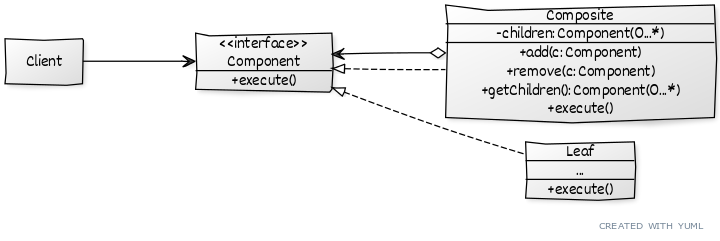
\includegraphics[width=0.8\linewidth]{images/CompositeUml}
	\caption{Diagram UML wzorca kompozyt.}
	\label{lab3/fig/CompositeUml}
\end{figure}
%[Client]->[Component]
%[Component]^-.-[Composite]
%[Composite]<>->[Component]
%[Component]^-.-[Leaf]
%
%[Client]
%[<<interface>>Component|+execute()]
%[Leaf|...|+execute()]
%[Composite|-children: Component(0...*)|+add(c: Component);+remove(c: Component);+getChildren(): Component(0...*);+execute()]

Jako przykład wykorzystania wzorca wyobraźmy sobie drzewo składające się z produktów oraz pudełek (kontenerów) które te produkty przechowują. Zarówno liście jak i kontenery implementują wspólny interfejs. Klient wywołuje metodę np. \texttt{GetPrice()} głównego kontenera (korzenia). Jeśli dzieckiem danego wierzchołka jest liść (produkt) zwracana jest jego cena, żądanie zostaje obsłużone bezpośrednio. Jeśli natomiast dzieckiem jest inny kontener (obiekt \texttt{Composite}), to przeglądana jest jego zawartość i ponownie w zależności od zawartości podejmowana jest akcja dotycząca dalszego przeglądania albo zwrócenia ceny.

Interfejsy graficzne, systemy SCADA zwykle pozwalają na rysowanie złożonych elementów z wielu innych, prostszych elementów. Klient nie chce traktować prostych i złożonych elementów w odmienny sposób. Powodowałoby to dodatkowe skomplikowanie modułu programu. Klasy \texttt{Line}, \texttt{Rectangle}, \texttt{Text} definiują proste elementy graficzne. Klasa \texttt{Picture} natomiast mogłaby stanowić kontener, w którym były przechowywane proste elementy podrzędne. Jest to jeden z przykładów, gdzie mógłby zostać wykorzystany wzorzec projektowy Kompozyt.

\subsubsection{Zadanie 2}

Jak w zadaniu pierwszym utwórz nowy projekt (aplikację konsolową .NET 5.0). Dodaj w nim folder o~nazwie \texttt{Equipments}. Wewnątrz tego folderu dodaj klasę abstrakcyjną komponentu \texttt{Equipment}\ref{lab3/lst/compositeAbstractClass}. Definiuje ona wspólny dla wszystkich klas interfejs. To po niej będą dziedziczyły klasy liści oraz kompozytów (kontenerów). Struktura drzewiasta będzie zawierała elementy komputera PC. Płyta główna i obudowa będą pełnić funkcję kontenerów natomiast procesor, pamięć RAM oraz dysk twardy będą pełnić funkcję liści.
\begin{lstlisting}[caption={Przykład abstrakcyjnej klasy komponentu}, label={lab3/lst/compositeAbstractClass}]
abstract class Equipment
{
	public abstract decimal NetPrice();
	public abstract decimal DiscountPrice();	
	public abstract int Power();
	public virtual void Add(Equipment component) => throw new NotImplementedException();	
	public virtual void Remove(Equipment component) => throw new NotImplementedException();
	public virtual bool IsComposite() => true;
}
\end{lstlisting}
%Normlanie lepiej byłoby zamiast stosować podstawowe typu utworzyć klasę Currency.
Następnie w tym samym projekcie dodaj klasy zarówno kontenerów np. \texttt{Chasis} oraz \texttt{Motherboard} oraz liści np. \texttt{Cpu}, \texttt{FloppyDisk}. Wszystkie powinny dziedziczyć po klasie \texttt{Equipment}. Przykładowa implementacja klasy \texttt{FloppyDisk} została pokazana na listingu~\ref{lab3/lst/compositeLeafFloppyDisk}.
\begin{lstlisting}[caption={Przykład klasy będącej liściem kompozytu}, label={lab3/lst/compositeLeafFloppyDisk}]
class FloppyDisk : Equipment
{
	private readonly decimal price;
	private readonly decimal discount;
	private readonly int power;
	
	public FloppyDisk(decimal price, decimal discount, int power)
	{
		this.price = price;
		this.discount = discount;
		this.power = power;
	}

	public override decimal NetPrice() => price;	
	public override bool IsComposite() => false;	
	public override decimal DiscountPrice() => price * (1 - discount);
	public override int Power() => power;
}
\end{lstlisting}
Klasa kontenera dodatkowo powinna posiadać pole listy na inne kontenery i liście oraz implementować metody wirtualne \texttt{Add} oraz \texttt{Remove}. Wspomniana lista może przechowywać zarówno obiekty kontenerów jak i~liści ponieważ oba typy dziedziczą po tej samej klasie abstrakcyjnej. Metody \texttt{NetPrice}, \texttt{DiscountPrice} oraz \texttt{Power} klasy kontenera powinny przeglądać dodane wcześniej komponenty (liście lub inne kontenery) i zwracać sumę cen wszystkich elementów podrzędnych. Fragment klasy \texttt{MotherBoardEquipment} wraz z~metodą zwracającą wartość będącą sumą cen wszystkich elementów pokazano na listingu~\ref{lab3/lst/compositeEquipmentClass}.
\begin{lstlisting}[caption={Fragment klasy \texttt{MotherBoardEquipment}}, label={lab3/lst/compositeEquipmentClass}]
class MotherBoardEquipment : Equipment
{
	protected List<Equipment> equipments = new List<Equipment>();

	//...
		
	public override void Add(Equipment component) => equipments.Add(component);	
	public override void Remove(Equipment component) => equipments.Remove(component);
	public override decimal NetPrice()
	{
		decimal result = price;
		equipments.ForEach(x => result += x.NetPrice());	
		return result;
	}
		
	//...
}
\end{lstlisting}

W klasie klienta, albo w metodzie \texttt{Main} sprawdź poprawność stworzonej struktury. Utwórz obiekt obudowy (\texttt{ChasisEquipment}) oraz dodaj do niego (za pomocą metody \texttt{Add}) kilka dysków twardych \texttt{FloppyDisk} oraz płytę główną \texttt{MotherBoardEquipment} do której wcześniej dodaj procesor \texttt{Cpu}.

Tak utworzoną strukturę przekaż do innej klasy klienckiej. Zwróć uwagę, że z punktu widzenia klienta nie ma znaczenia czy korzysta on z pojedynczego elementu liścia (np. klasy reprezentującej procesor) czy z~kontenera, który zawiera wiele dodatkowych elementów podrzędnych. Złożoność struktury drzewiastej jest przed nim ukryta przy pomocy wzorca Kompozyt.
\begin{lstlisting}
class Client
{
	public void PrintBill(Equipment equipment)
	{
		Console.WriteLine($"Bill:\n\t{equipment.NetPrice()}\n\t{equipment.DiscountPrice()}\n\t{equipment.Power()}");
	}
}
\end{lstlisting}

\subsection{Fasada (ang. facade)}\label{lab3/sec/FacadeUml}
Jeśli istnieje potrzeba, aby ukryć złożoność całej biblioteki albo pewnego zbioru wielu klas można użyć wzorca projektowego Fasada (diagram UML przedstawiono na rysunku~\ref{lab3/fig/FacadeUml}). Jest to wzorzec upraszczający sposób w jaki klienci korzystają z współpracujących, zależnych od siebie klas. Fasada udostępnia jednolity interfejs dla zbioru interfejsów z podsystemu. Wykorzystując Fasadę klient nie musi tworzyć, ani zarządzać zależnościami pomiędzy obiektami, są one przed nim ukryte za interfejsem Fasady. Wzorzec ten może również służyć za punkt wejścia dla podsystemu w~warstwowo podzielonym zestawie.

Fasada pozwala zmniejszyć liczbę obiektów z której korzystają klienci. Dodatkowo wprowadza luźne powiązanie pomiędzy klientami, a podsystemami. Ułatwione jest dzięki temu wprowadzanie zmian w~podsystemach jak również zmiana zależności między nimi. 

\begin{figure}[hbt!]
	\centering
	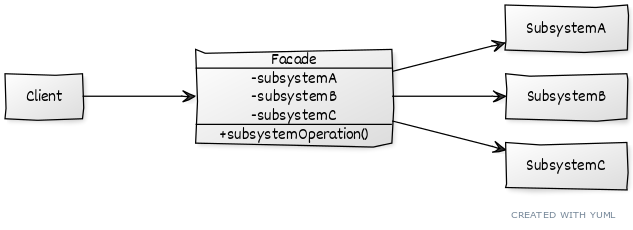
\includegraphics[width=0.8\linewidth]{images/FacadeUml}
	\caption{Diagram UML wzorca Fasada.}
	\label{lab3/fig/FacadeUml}
\end{figure}
%[Client]->[Facade]
%[Facade]->[SubsystemA]
%[Facade]->[SubsystemB]
%[Facade]->[SubsystemC]
%
%[Client]
%[Facade|-subsystemA;-subsystemB;-subsystemC|+subsystemOperation()]
%[SubsystemA]
%[SubsystemB]
%[SubsystemC]

Interfejs udostępniany przez omawiany wzorzec jest uproszczony. Klasa Fasady nie musi korzystać z~wszystkich funkcjonalności klas, które wykorzystuje. Dostarczane są jedynie te niezbędne. 
%Jedynie bardziej wymagający klienci będą musieli spojrzeć za fasadę.

Przykładem zastosowania Fasady może być ukrycie złożoności procesu konwersji materiału wideo. Klient \textbf{nie} korzystający z omawianego wzorca byłby zmuszony do wykorzystywania różnych klas. Inna klasa zostałaby użyta do kompresji materiału wideo inna do miksowania audio, a jeszcze inna do zmiany formatu pliku. Klient może potrzebować jedynie uproszczonego interfejsu do konwertowania pliku wideo. Nie interesują go złożone mechanizmy tego procesu. Dlatego zamiast zmuszać klienta do posiadania i zarządzania wieloma klasami, można utworzyć klasę fasady, która te złożoności przed nim ukryje. Jeśli w przyszłości część wykorzystywanych klas się zmieni, aktualizacja kodu będzie wymagana tylko w klasie Fasady.

Innym przykładem, gdzie omawiany wzorzec ma zastosowanie jest podsystem kompilujący. Również w~tym przypadku klienta nie interesują złożone zależności pomiędzy parserem, preprocesorem, analizatorem semantyki czy optymalizatorem. Autorzy klientów chcą tylko skompilować kod. Jeśli proces kompilacji zostanie ukryty w~pojedynczej klasie \texttt{Compiler}, to będzie ona odgrywała rolę fasady.
% g++ -Wall -std=c++14 main.cpp -o main.exe //-Wall (all warnings) and -o main.exe instead of a.exe

\subsubsection{Zadanie 3}

Utwórz kolejny projekt w~analogiczny jak w poprzednich zadaniach sposób. Tym razem zostanie wykorzystany wzorzec projektowy Fasady do ukrycia złożoności serwisów odpowiedzialnych za pobieranie informacji o ,,danych meteorologicznych''.

Dodaj do projektu folder \texttt{WeatherServices}. Następnie umieść w nim trzy interfejsy w osobnych plikach: \texttt{ITemperatureService}, \texttt{IHumidityService} oraz \texttt{IForecastService}. Każdy z nich niech deklaruje jedną metodę: \texttt{double GetTemperature()}, \texttt{double GetHumidity()} i \texttt{double GetForecast()}. 

Dodaj do tego samego folderu trzy klasy implementujące te interfejsy. W celu wygenerowania pomiarów możesz skorzystać z~generatora liczb pseudolosowych np. klasy \texttt{System.Random} i jej metody \texttt{NextDouble}. Generacja liczb z pewnego przedziału może być zrealizowana w następujący sposób:
\begin{lstlisting}	
random.NextDouble() * (maxValue - minValue) + minValue;
\end{lstlisting}
%To generate a cryptographically secure random number, such as one that's suitable for creating a random password, use the RNGCryptoServiceProvider class or derive a class from System.Security.Cryptography.RandomNumberGenerator.
Można również wykorzystać Metodę Rozszerzającą (ang. Extension Method)\footnote{Metody rozszerzające pozwalają na ,,dodanie'' metody do już istniejącego typu, bez konieczności tworzenia nowej klasy pochodnej czy modyfikacji klasy już istniejącej. Metody rozszerzające są statyczne, ale ich wywołanie wygląda jakby należało do instancji danej klasy. Kompilator tłumaczy wywołanie tej metody na metodę statyczną. 
% Enkapsulacja nie jest naruszona, metody rozszerzajace nie maja dostepu do składowych prywatnych.
}. Dodaj do projektu folder \texttt{Extensions}, a w nim statyczną klasę \texttt{RandomExtension}. W  klasie natomiast dodaj statyczną metodę \texttt{NextDouble} o następującej postaci:
\begin{lstlisting}	
public static class RandomExtensions
{
	public static double NextDouble(this Random random, double minValue, double maxValue)
	{
		return random.NextDouble() * (maxValue - minValue) + minValue;
	}
}
\end{lstlisting}
Zwróć uwagę na pierwszy parametr, określa on do jakiego typu (klasy) chcemy ,,dodać'' nową metodę. Konieczne jest, aby poprzedzić go słowem kluczowym \texttt{this}. Kolejne parametry nie różnią się niczym od tych ze standardowej deklaracji metody.

Po dodaniu klasy \texttt{RandomExtension} klasa \texttt{Random} ,,otrzymała'' nową metodę, która generuje liczbę pseudolosową typu \texttt{double} z określonego przez klienta przedziału. Metod rozszerzających nie należy stosować tam gdzie możemy modyfikować kod klasy, dodać składową. Jest to jednak dobre narzędzie jeśli chcemy dodać funkcjonalność do kodu, który nie jest pod naszą kontrolą, a dziedziczenie jest nieodpowiednie albo niemożliwe. 

Klasy implementujące utworzone wcześniej interfejsy mogą teraz wykorzystywać metody rozszerzające. Listing~\ref{lab3/lst/temperatureServiceExtensionMethod} przedstawia przykładową implementację klasy \texttt{TemperatureService}.
\begin{lstlisting}[caption={Fragment klasy \texttt{TemperatureService} wykorzystującej metodę rozszerzającą}, label={lab3/lst/temperatureServiceExtensionMethod}]	
public class TemperatureService : ITemperatureService
{
	public double GetTemperature() => new Random().NextDouble(-20, 40);
}
\end{lstlisting}

Dalej dodaj do głównego katalogu projektu plik z rekordem\footnote{Słowo kluczowe \texttt{record} wraz z \texttt{init} pojawiło się C\# 9.0 i pozwala zdefiniować typ referencyjny, który służy do przechowywania danych. Tworzone w ten sposób typ jest \textbf{niezmienny} tzn. stan takiego obiektu nie może się zmienić po jego utworzeniu. Zmiana jego stanu jest możliwa jedynie poprzez utworzenie nowej instancji. Rekordy pozwalają na utworzenie nowego obiektu bez konieczności przepisywania wszystkich właściwości, jedna po drugiej. Można posłużyć się słowem kluczowym \texttt{with} i zmienić jedną właściwość, pozostałe zostaną natomiast przepisane automatycznie. Przed pojawieniem się rekordów konieczne było tworzenie właściwości jedynie z akcesorem \texttt{get} oraz ustawianie ich w konstruktorze za pomocą przekazanych przez klienta argumentów.} \texttt{Weather}:
\begin{lstlisting}	
public record Weather(double Temperature, double Humidity, double Forecast);
\end{lstlisting}

Umieść z katalogu głównym nową klasę Fasady dla wcześniej stworzonych serwisów. Klasa Fasady niech zawiera trzy pola w których przechowasz referencję do obiektów implementujących utworzone wcześniej interfejsy. W konstruktorze przypisz im przekazane przez parametry konstruktora obiekty. Dodaj również metodę \texttt{GetWeatherInformation} zwracającą obiekt typu \texttt{Weather}. Metoda ta niech pobiera informacje o~temperaturze, wilgotności oraz estymacji przekazanych serwisów i zwraca jeden obiekt zawierający te dane:
\begin{lstlisting}	
public class WeatherApiFasade
{
	//...
	
	public WeatherApiFasade(ITemperatureService temperatureService, 
		IHumidityService humidityService, IForecastService forecastService)
	{
		//...
	}
	
	public Weather GetWeatherInformation()
	{
		return  new(
			temperatureService.GetTemperature(),
			humidityService.GetHumidity(),
			forecastService.GetForecast());
	}
}
\end{lstlisting}

Na koniec dodaj do projektu klasę \texttt{Application}:
\begin{lstlisting}	
class Application
{
	public static void Run(WeatherApiFasade weatherApiFasade)
	{
		Console.Write(weatherApiFasade.GetWeatherInformation());
	}
}
\end{lstlisting}
W metodzie \texttt{Main} utwórz obiekt typu \texttt{WeatherApiFasade} przekazując do niego wcześniej utworzone obiekty wymagane przez konstruktor. Wywołaj metodę \texttt{Run()} i sprawdź czy na ekranie konsoli zostały wypisane oczekiwane wyniki:
\begin{lstlisting}	
static void Main(string[] args)
{
	WeatherApiFasade weatherApiFasade = new WeatherApiFasade(
		new TemperatureService(), 
		new HumidityService(),
		new ForecastService());
	
	Application.Run(weatherApiFasade);
}
\end{lstlisting}
